\section{Architecture of model checker}\label{sec:methods}
In this section, we will explore the methods used for model checking confidentiality and integrity policies. In \autoref{sec:data-repository} the notion of policy formulae and a transformation from these formulae to LTL were introduced. This transformation to LTL allows formal, well-known model checking algorithms to be applied to said formulae. This section will present a model checking approach based on transforming the negated formula into a Büchi automaton. This is performed in two steps, first constructing the Generalised Nondeterministic Büchi Automaton (GNBA) and then transforming the GNBA into an equivalent Nondeterministic Büchi Automaton (NBA). The product of the NBA and the transition system (the data repository) can then be checked for the persistence property by a nested depth-first search. In \autoref{fig:model-checker} an overview of the process is shown, where the figure is inspired by~\cite[Fig.~5.16]{baier2008principles}.

\begin{figure}[!ht]
    \centering
    \begin{center}
        \begin{tikzpicture}[node distance=2cm,scale=0.75, every node/.style={scale=0.75}]
        \tikzstyle{startstop} = [rectangle, rounded corners, minimum width=3cm, minimum height=1cm,text centered, draw=black]
        \tikzstyle{process} = [rectangle, minimum width=4.1cm, minimum height=1cm, text centered, text width=4.1cm, draw=black,fill=white!20]
        \tikzstyle{arrow} = [thick,->,>=stealth]
        
        \node[]             (text)      at (0,3.7)      {Model checker};
        
        % Left side
        \node[startstop]    (start1)    at (-3.9,9.5)   {Data repository DR};
        \node[process]      (dr)        at (-3.9,6.5)   {Model of system DR};
        \node[process]      (drtots)    at (-3.9,5)     {Transformation from DR to TS \autoref{def:dr-to-ts}};
        \node[process]      (ts)        at (-3.9,3.5)   {Transition system TS};
        
        % Right side
        \node[startstop]    (start2)    at (3.9,9.5)    {User policy formula $\upf$};
        \node[process]      (upftoipf)  at (3.9,8)      {Transformation from UPF to IPF $\pf$, \autoref{def:pf-user-to-internal}};
        \node[process]      (ipftoltl)  at (3.9,6.5)    {Transformation from IPF to LTL $\phi$, \autoref{def:pf-to-ltl}};
        \node[process]      (ltl)       at (3.9,5)      {Negation of LTL-formula $\lnot \phi$};
        \node[process]      (gnba)      at (3.9,3.5)    {Generalised Büchi automaton};
        \node[process]      (nba)       at (3.9,1.5)    {Büchi automaton $\mathcal{A}_{\lnot \phi}$};
        
        % Middle
        \node[process]      (product)   at (0,0)        {Product transition system $TS \otimes \mathcal{A}_{\lnot \phi}$};
        \node[process]      (sat)       at (0,-1.5)     {$TS \otimes \mathcal{A} \models P_{pers(\mathcal{A}_{\lnot \phi})}$};
        \node[startstop]    (yes)       at (-3.9,-3)    {Yes};
        \node[startstop]    (no)        at (3.9,-3)     {No};
       
        % Left side
        \draw[arrow] (start1)      --    (dr);
        \draw[arrow] (dr)          --    (drtots);
        \draw[arrow] (drtots)      --    (ts);
        \draw[arrow] (ts)          |-    (product);
        
        % Right side
        \draw[arrow] (start2)      --    (upftoipf);
        \draw[arrow] (upftoipf)    --    (ipftoltl);
        \draw[arrow] (ipftoltl)    --    (ltl);
        \draw[arrow] (ltl)         --    (gnba);
        \draw[arrow] (gnba)        --    (nba);
        \draw[arrow] (nba.south)   |-    (product.east);
        
        % Middle
        \draw[arrow] (product)     --    (sat);
        \draw[arrow] (sat.west)    -|    (yes.north);
        \draw[arrow] (sat.east)    -|    (no.north);
        
        \begin{pgfonlayer}{background}
            \filldraw [draw=black,fill=black!10](ts.north -| gnba.east)+(0.2,0.2) rectangle ([shift={(-0.2,-0.2)}] sat.south -| ts.west);
        \end{pgfonlayer}
    \end{tikzpicture}
\end{center}
    \caption{Overview of PF model checking.}
    \label{fig:model-checker}
\end{figure}

This section will also cover an optimized approach of finding elementary sets and a short introduction on how to parse policy formulae from a text-based representation into an abstract syntax tree.

\subsection{Parsing LTL formulae}
Parsing an LTL formula from a text-based representation into an abstract syntax tree (AST) is performed using a top-down parser with the recursive descent algorithm. The recursive descent algorithm follows the structure of the context-free grammar closely by having a mutually exclusive procedure for each non-terminal production rule in the grammar. Care has to be taken to uphold the left- and right-associative rules for each of the operators. In \autoref{alg:recursive-descent} the overall structure of the recursive descent algorithm can be seen for the $i$'th production rule.
\begin{algorithm}[H]
\SetAlgoLined
\DontPrintSemicolon
\SetKwProg{rd}{Algorithm}{}{}
\rd{$rd_i()$}{
    $lhs := rd_{i+1}()$\;
    \If{$token \in scanner$}{
        \KwRet $op\{lhs, rd_i()\}$
    }
    \KwRet lhs
}{}

\caption{The recursive descent algorithm for the $i$'th production rule.}
\label{alg:recursive-descent}
\end{algorithm}
A procedure for the $i'th$ production rule generally parses its left-hand side with the production rule immediately following itself, i.e. the production rule with immediate higher associativity. The procedure then recurses on the right-hand side, as long as the operator matching the current production rule can be found in the input stream. Recursing on the right-hand side makes the parsing right-associative. 

\begin{example}
We consider the AST for the formula $\phi \eqdef a \U b \land c$ which can be seen in \autoref{fig:ast-exampl1}. The precedence rule of the until operator ($\U$) is stronger than that of the conjunction ($\land$), which is explicitly shown in the AST.
\begin{figure}[!ht]
    \centering
    \begin{forest}
for tree={draw, minimum size=5mm, anchor=center}  
[$\land$,
    [$\U$,
        [$a$]
        [$b$]
    ]
    [$c$]
]
\end{forest}
    \caption{The AST for $\phi \eqdef a \U b \land c$.}
    \label{fig:ast-exampl1}
\end{figure}
\end{example}

\begin{example}
We consider the AST for the formula $\phi \eqdef a \U b \U c$ which can be seen in \autoref{fig:ast-exampl2}. Because the until operator ($\U$) is right-associative, which is conveyed by the AST, the subformula $b \U c$ is evaluated first, and therefore not the root of the tree.

\begin{figure}[!ht]
    \centering
    \begin{forest}
        for tree={draw, minimum size=5mm, anchor=center}  
        [$\U$,
            [$a$]
            [$\U$,
                [$b$]
                [$c$]
            ]
        ]
    \end{forest}
    \caption{The AST for $\phi \eqdef a \U b \U c$.}
    \label{fig:ast-exampl2}
\end{figure}
\end{example}

\subsection{Determining Elementary Sets}
\label{sec:method-elemesets}
The problem of finding elementary sets is essential in model checking of LTL formulae. In this paper two methods are presented for determining the elementary sets of an LTL formula, the first being a naive approach and the second being an optimized decision tree-based approach.

\subsubsection{Naive approach}
In the naive approach for finding elementary sets all subsets of the closure of $\phi$ are considered to be elementary or not. Since all subsets of $closure(\phi)$ are considered, the naive approach does not exclude any sets which are trivially not elementary, i.e. sets which are not maximal. Since $|closure(\phi)|$ is $\mathcal{O}(|\phi|)$ the number of possible elementary sets which is considered by the naive approach is $\mathcal{O}(2^{|\phi|})$. Checking whether a set is elementary or not takes $\mathcal{O}(|\phi|)$ time which results in a total time complexity of $\mathcal{O}(2^{|\phi|} \cdot |\phi|)$. The algorithm is correct since all sets are considered.

\subsubsection{Decision tree approach}\label{sec:methods-dt}
The decision tree based approach exploits the property of elementary sets being maximal, i.e. for all $\psi \in closure(\phi)$:
\begin{equation*}
  \psi \notin B \imply \lnot \psi \in B \tag{\autoref{eq:elem3.1}}
\end{equation*}
This very fundamental property leads to a binary relationship for each subformula, where either the negated or the non-negated subformula must be present in the elementary set. The algorithm considers all subformulae $\psi$ of $\phi$ in ascending order of their formula length $|\psi|$. This results in the smallest subformulae being considered prior to any other subformula.

The algorithm recursively explores a decision tree where a node at depth $i$ will have one edge exploring the $i$'th subformula of $\phi$ and another edge exploring the negation of that subformula. A node is marked inconsistent if the path $\pi$ from the root node to the node itself (corresponding to a set of subformulae) is inconsistent with respect to the properties for elementary sets. An inconsistent node halts further exploration, as an inconsistent node can not reach a state where the path becomes consistent again. The decision tree is complete when all subformulae of $\phi$ have been considered. The definition for constructing a decision tree is provided in the following:
\begin{definition}[Decision Tree Algorithm for Elementary Sets (DT)]
Let $\phi$ be an LTL formula and $\vec{f}$ be the partial order of subformulae $\psi$ of $\phi$ sorted according to $|\psi|$. Let $DT: F^\ast, 2^F \rightarrow T$ be the definition for the decision tree algorithm where $F$ is the set of all possible LTL formulae and $T$ all possible decision trees. The tree is constructed from three types of nodes, given the following definition:
\begin{align*}
    \begin{forest}
    for tree={circle, draw}
    [, 
    ]
\end{forest} &\text{ is a root or intermediate node} \\
    \begin{forest}
    for tree={circle, draw}
    [,cross out 
    ]
\end{forest}  &\text{ is an inconsistent node} \\
    \begin{forest}
    for tree={circle, draw, square/.style={regular polygon,regular polygon sides=4}}
    [,square
    ]
\end{forest} &\text{ is a terminal node}
\end{align*}
Now construct the decision tree $DT(\vec{f}, \varnothing)$ given by the following definition:
\begin{align*}
    DT(\epsilon, \lambda) &= 
        \begin{cases}
            \begin{tabular}{ m{2cm} m{3cm} }
    \hspace*{-0.14in}
    \centering{\begin{forest}
    for tree={circle, draw, square/.style={regular polygon,regular polygon sides=4}}
    [,square
    ]
\end{forest}}
    &
        $\text{if } \Delta (\lambda)$
    \\
    \hspace*{-0.14in}
    \centering{\begin{forest}
    for tree={circle, draw}
    [,cross out 
    ]
\end{forest}}
    &
        $\text{if } \lnot \Delta (\lambda)$
    \\
\end{tabular}
        \end{cases}
    \\
    DT(f \tcdot \vec{f}, \lambda) &= 
        \begin{cases}
        \begin{tabular}{ m{2cm} m{3cm} }
    \centering{\begin{forest}
for tree={circle, draw, s sep=14pt}
[,
    [,label={[yshift=-4mm,]$lhs$}, draw=none, edge label={node[midway,left] {$f$}} ]
    [,label={[yshift=-4mm,]$rhs$},draw=none, edge label={node[midway,right] {$\lnot f$}} ]
]
\end{forest}}
    &
    \begin{equation*}
        \begin{gathered}
        \text{if } \Delta (\lambda) \enskip \land \\
        lhs=DT(\vec{f}, \lambda \cup \{f\})\enskip\land \\
        rhs=DT(\vec{f}, \lambda \cup \{\lnot f\})
        \end{gathered}
    \end{equation*}
    \\
    \hspace*{-0.14in}
    \centering{\begin{forest}
    for tree={circle, draw, s sep=14pt}
    [,cross out 
    ]
\end{forest}}
    &
    \begin{equation*}
        \begin{gathered}
        \text{if } \lnot \Delta (\lambda)
        \end{gathered}
    \end{equation*}
    \\
\end{tabular}
        \end{cases}
\end{align*}
where $\Delta: 2^F \rightarrow \mathbb{B}$ is the function determining inconsistency of paths given by the following definition:
\begin{align*}
    \Delta(\lambda) =
    \begin{cases}
        true & \text{if $\lambda$ is elementary w.r.t. $closure(\lambda)$} \\
        false & \text{otherwise}
    \end{cases}
\end{align*}
We note here that $closure(\lambda)$ denotes set set of all formulae in $\lambda$ and their negations. Furthermore the elementary set properties are defined in \autoref{eq:elem1.1}~-~\autoref{eq:elem3.1}. Lastly, let $P$ be all paths in $DT(\vec{f}, \varnothing)$ from the root node to a terminal node. Then the elementary sets of $\phi$ is the sets of edge labels for all paths in $P$.

For readability we denote the decision tree of $\phi$ as $DT_\phi$.
\end{definition}

Since the height of the decision tree is $\mathcal{O}(|\phi|)$ and the tree is binary, the time complexity for exploring the decision tree is $\mathcal{O}(2^{|\phi|})$. Although the time complexity is still exponential with respect to $|\phi|$, as the naive approach, in practice the algorithm shows vast improvements because of the early elimination of inconsistent nodes, as shown later in this section. For completeness, we provide the following proof for the correctness of the DT algorithm. First, we introduce some essential properties of $DT_\phi$ which are required for the proof.

\begin{definition}[Properties of paths of $DT_\phi$]
\label{def:dt-props}
Let $\lambda$ be the set of subformulae on the path $\pi$ in a decision tree $DT_\phi$. Then the following holds:
\begin{enumerate}[label=(\alph*)]
    \item \label{def:dt-prop1} $\phi \in \lambda \imply \phi \in closure(\lambda)$
    \item \label{def:dt-prop2} $\phi \in closure(\phi) \imply \phi \in \lambda \oplus \lnot \phi \in \lambda$
    \item \label{def:dt-prop3} $\phi_1 \in closure(\lambda) \land |\phi_1| > |\phi_2| \imply \phi_2 \in closure(\lambda)$
\end{enumerate}
\end{definition}

\begin{proof}
We start of by proving that for any consistent path $\pi=\pi_0,\ldots,\pi_n$ in the decision tree $DT_\phi$, the set $\lambda$ consisting of the subformulae on the path of $\pi$ is an elementary set with respect to $closure(\lambda)$. A consistent path is any path containing no inconsistent nodes and by $closure(\lambda)$ we denote all subformulae in $\lambda$ and their negations. In the following we show that \autoref{eq:elem1.1}, \autoref{eq:elem1.3}, \autoref{eq:elem2.1} and \autoref{eq:elem2.2} holds because of the partial order of $\vec{f}$ and the definition for elementary sets (\autoref{sec:elemesets}). The remaining properties, \autoref{eq:elem1.2} and \autoref{eq:elem3.1} is later proven by the structure of the decision tree.

We start by considering \autoref{eq:elem1.1}. Assume that, for a consistent path $\pi$, this property does not hold for~$\lambda=B$ with respect to $closure(\lambda)$. Then we must have one of two scenarios:
\begin{itemize}
    \item $\phi_1 \land \phi_2 \in B \land \lnot(\phi_1 \in B \text{ and } \phi_2 \in B)$ \quad
    Because of the ordering of $\vec{f}$ and that $|\phi_1 \land \phi_2| < |\phi_1|$ and $|\phi_1 \land \phi_2| < |\phi_2|$, we know that $\phi_1 \land \phi_2 \in B \imply \phi_1 \in B \oplus \lnot\phi_1 \in B \land \phi_2 \in B \oplus \lnot\phi_2 \in B$ using \autoref{def:dt-props}. Then if $\phi_1 \notin B$ or $\phi_2 \notin B$ we have $\lnot\Delta(\lambda)$ and thus $\pi$ can not be consistent. This contradicts the assumption.
    %Otherwise the path would contain an inconsistent node. This contradicts the assumption.
    \item $\phi_1 \land \phi_2 \notin B \land \phi_1 \in B \land \phi_2 \in B$ \quad We know that $\phi_1 \land \phi_2 \in closure(\lambda)$ but $\phi_1 \land \phi_2 \notin B$. Because $\phi_1 \in B$ and $\phi_2 \in B$ this case is trivially a contradiction since $\lnot\Delta(\lambda)$ and thus $\pi$ would contain an inconsistent node.
\end{itemize}
\autoref{eq:elem1.3} is trivial and can be proven in a similar manner. We now proceed to consider \autoref{eq:elem2.1}. Assume that, for a consistent path $\pi$, this property does not hold for $\lambda=B$ with respect to $closure(\lambda)$. Then we must have the following scenario:
\begin{itemize}
    \item $\phi_2 \in B \land \phi_1 \U \phi_2 \notin B$ \quad
    Again we exploit the ordering of $\vec{f}$. We therefore know $\phi_2$ to be on the path prior to $\phi_1 \U \phi_2$. If $\phi_1 \U \phi_2 \notin B$ then $\lnot\Delta(\lambda)$ and thus $\pi$ would contain an inconsistent node. This contradicts our assumption.
\end{itemize}
Lastly we consider \autoref{eq:elem2.2}. Assume that, for a consistent path $\pi$, this property does not hold for $\lambda=B$ with respect to $closure(\lambda)$. Then we have the following scenario:
\begin{itemize}
    \item $\phi_1 \U \phi_2 \in B \land \phi_2 \notin B \land \phi_1 \notin B$ \quad Again, because of the ordering of $\vec{f}$, $\phi_1$ and $\phi_2$ must appear on the path $\pi$ prior to $\phi_1 \U \phi_2$. If $\phi_1 \notin B$ or $\phi_2 \notin B$, then this path would contain an inconsistent node. This contradicts our assumption.
\end{itemize}

It now remains to show that \autoref{eq:elem1.2} and \autoref{eq:elem3.1} holds under the structure of the decision tree. We prove this by contradiction. Assume that \autoref{eq:elem1.2} does not hold for some path $\pi$, meaning:
\begin{equation*}
    \psi \in B \land \lnot \psi \in B \tag{contradiction of \ref{eq:elem1.2}}
\end{equation*}
Then $\psi$ and $\lnot \psi$ must belong to some edge $\pi_i \in \pi$ and $\pi_j \in \pi$. Since $\psi$ and $\lnot\psi$ must be an edge on the same depth in the decision tree, i.e. $i=j$, $\psi$ and $\lnot \psi$ must be in two different subtrees, thus $\pi$ can not contain both. More formally this is proven using \autoref{def:dt-props} which states that $\psi \in B \oplus \lnot\psi \in B$. This contradicts our assumption.

For the case of maximality, we again consider the following contradiction. Assume that the rule of maximality, \autoref{eq:elem3.1}, does not hold, meaning:
\begin{equation*}
    \psi \notin B \land \lnot \psi \notin B \tag{contradiction of \ref{eq:elem3.1}}
\end{equation*}
Then $\psi \notin \pi$ and $\lnot\psi \notin \pi$. However we know that $\psi \in closure(\lambda)$ and thus either $\psi \in \pi$ or $\lnot\psi \in \pi$ following \autoref{def:dt-props}. This contradicts our assumption.

Because we have shown the elementary set properties to hold for $\lambda$  with respect to $closure(\lambda)$ of any consistent path $\pi$, we lastly note that any path $\pi$ of length $|\vec{f}|$ has $closure(\lambda)=closure(\phi)$ for at decision tree $DT_\phi$. This concludes that every $\lambda$ for all consistent paths $\pi$ of length $|\vec{f}|$ is an elementary set with respect to $closure(\phi)$.
\end{proof}

\begin{example}
We now consider the decision tree $DT_\phi$ for $\phi \eqdef a \cup (a \land b)$. In figure~\ref{fig:elemset} the fully explored decision tree can be seen.

\begin{figure}[!ht]
\begin{center}
    \begin{forest}
for tree={circle, draw, s sep=14pt}
[, 
    [,edge label={node[midway,left] {$a$}}  
      [,edge label={node[midway,left] {$b$}}
        [,edge label={node[midway,left] {$a \land b$}}
            [,edge label={node[midway,left] {$\varphi$}}]
            [,cross out, edge label={node[midway,right] {$\lnot\varphi$}}]
        ]
        [,cross out, edge label={node[midway,right] {$\lnot (a \land b)$}}
            [,draw=none,edge={draw=none}]
            [,draw=none,edge={draw=none}]
        ] 
      ] 
      [,edge label={node[midway,right] {$\lnot b$}}
        [,cross out, edge label={node[midway,left] {$a \land b$}}
            [,draw=none,edge={draw=none}]
            [,draw=none,edge={draw=none}]
        ] 
        [, edge label={node[midway,right] {$\lnot (a \land b)$}}
            [,edge label={node[midway,left] {$\varphi$}}]
            [,edge label={node[midway,right] {$\lnot\varphi$}}]
        ] 
      ] 
    ]
    [,edge label={node[midway,right] {$\lnot a$}}
      [,edge label={node[midway,left] {$b$}}
        [,cross out, edge label={node[midway,left] {$a \land b$}}
            [,draw=none,edge={draw=none}]
            [,draw=none,edge={draw=none}]
        ]
        [,edge label={node[midway,right] {$\lnot (a \land b)$}}
            [,cross out, edge label={node[midway,left] {$\varphi$}}]
            [,edge label={node[midway,right] {$\lnot\varphi$}}]
        ] 
      ] 
      [,edge label={node[midway,right] {$\lnot b$}}
        [,cross out, edge label={node[midway,left] {$a \land b$}}
            [,draw=none,edge={draw=none}]
            [,draw=none,edge={draw=none}]
        ]
        [,edge label={node[midway,right] {$\lnot (a \land b)$}}
            [,cross out, edge label={node[midway,left] {$\varphi$}}]
            [,edge label={node[midway,right] {$\lnot\varphi$}}]
        ]
      ]  
  ] 
]
\end{forest}
    \caption{Decision tree $DT_\phi$ for formula $\phi = a \U (a \land b)$.}
    \label{fig:elemset}
\end{center}
\end{figure}

After the exploration of the decision tree, one can find the elementary sets of $\phi$ as all paths in $DT_\phi$ from the root reaching a terminal node. This results in the following elementary sets:
\begin{align*}
    B_1 &= \{a,         b,         a\land b,           \phi\} \\
    B_2 &= \{a,         \lnot b,    \lnot (a\land b),   \phi\} \\
    B_2 &= \{a,         \lnot b,    \lnot (a\land b),   \lnot \phi\} \\
    B_4 &= \{\lnot a,   b,         \lnot (a\land b),  \lnot \phi\} \\
    B_5 &= \{\lnot a,   \lnot b,    \lnot (a\land b),   \lnot \phi\} \\
\end{align*}
\end{example}

\paragraph{Performance comparison}
The formulae in \autoref{tab:elem-test} is a subset of the formulae used in \cite[Tab.~1]{somenzi2000efficient} for testing their algorithm for creating Büchi automaton from LTL formulae. In the table, the mean time of execution is shown for each formula, i.e. the mean time it takes to produce the elementary set.

\begin{table}[!ht]
    \centering
    \makeatletter
           \def\rulecolor#1#{\CT@arc{#1}}
           \def\CT@arc#1#2{%
           \ifdim\baselineskip=\z@\noalign\fi
           {\gdef\CT@arc@{\color#1{#2}}}}
           \let\CT@arc@\relax
          \rulecolor{gray!50}
        \makeatother
    \begin{tabular}{@{}llll@{}}
        \toprule
        Formula $\phi$ & Naive & DT & Improvement \\ 
        \cmidrule(r){1-1}\cmidrule(lr){2-2}\cmidrule(lr){3-3}\cmidrule(l){4-4}
        $p \U q$                                                                                    & 2.27~µs    & 129~µs     & 17.5x \\
        $p \U (q \U r)$                                                                             & 125~µs     & 33.6~µs    & 3.73x \\
        $\lnot(p \U (q \U r))$                                                                      & 2.63~ms    & 174~µs     & 15.1x \\
        $\G \F p \imply \G \F q$                                                                    & 46.7~ms    & 1.42~ms    & 32.9x \\
        $\F  p \U \G q$                                                                             & 2.40~ms    & 190~µs     & 12.7x \\
        \midrule
        $\G  p \U q$                                                                                & 515~µs     & 78.6~µs    & 6.55x \\
        $\lnot(\G \F p \imply \G \F q)$                                                             & 47.9~ms    & 1.76~ms    & 27.3x \\
        $(\X (p) \U \X (q)) \lor \lnot \X (p \U q)$                                                 & 267~ms     & 1.70~ms    & 157x \\
        $(\X (p) \U q) \lor \lnot \X (p \U (p \land q))$                                            & 307~ms     & 1.20~ms    & 255x \\
        $\G  (p \imply \F  q) \land ((\X (p) \U q) \lor \lnot \X (p \U (p \land q)))$               & 214~s      & 25.0~ms    & 8529x \\
        \midrule
        $\G  (p \imply \F  q) \land ((\X (p) \U \X (q)) \lor \lnot \X (p \U q))$                    & 297~s      & 34.2~ms    & 8685x \\
        $\G  (p \imply \F  q)$                                                                      & 2.80~ms    & 262~µs     & 10.7x \\
        $\lnot (\G \F p \lor \F \G q)$                                                              & 47.9~ms    & 1.75~ms    & 27.3x \\
        $\G  (\F  p \land \F  q)$                                                                   & 10.9~ms    & 404~µs     & 27.0x \\
        $\F  p \land \F  \lnot p$                                                                   & 591~µs     & 83.3~µs    & 7.09x \\
        \midrule
        $(\G  (q \lor \G \F p) \land \G  (r \lor \G \F  \lnot p)) \lor \G  q \lor \G  r$            & N/A        & 1.62~s     & N/A \\
        $(\G  (q \lor \F \G p) \land \G  (r \lor \F \G  \lnot p)) \lor \G  q \lor \G  r$            & N/A        & 1.62~s     & N/A \\
        $\lnot ((\G  (q \lor \G \F p) \land \G  (r \lor \G \F  \lnot p)) \lor \G  q \lor \G  r)$    & N/A        & 2.01~s     & N/A \\
        $\lnot ((\G  (q \lor \F \G p) \land \G  (r \lor \F \G  \lnot p)) \lor \G  q \lor \G  r)$    & N/A        & 2.05~s     & N/A \\
        $\G  (q \lor \X \G p) \land \G  (r \lor \X \G  \lnot p)$                                    & 213~s      & 66.3~ms    & 3217x \\
        \midrule
        $\G  (q \lor (\X p \land \X  \lnot p))$                                                     & 60.0~ms    & 1.08~ms    & 55.3x \\
        $(p \U p) \lor (q \U p)$                                                                    & 2.46~ms    & 107~µs     & 23.0x \\
        \bottomrule
        Total                                                                                       & 725~s      & 7.44~s     & 97.5x
 \\
        \bottomrule
    \end{tabular}
    \caption{Comparison of the naive approach and the decision tree approach of determining elementary sets. For each formula the mean time of execution is given. Results are performed on a desktop computer with a Intel\textsuperscript{\textregistered} Core\texttrademark~i7-950 processor. Results shown as \emph{N/A} were infeasible to compute because of resource constraints.}
    \label{tab:elem-test}
\end{table}

In most cases, the decision tree-based approach delivers significantly faster results compared to the naive approach. Only in one of the tested cases, the naive outperforms the decision tree approach. The formula tested in this case only had length 1, so there are only a few sets to consider if they are elementary or not. In other cases, the naive approach is not able to terminate, because the system is out of memory or exceeds the time limitation of 10 minutes. Furthermore, in three cases the naive approach uses more than 200 seconds, which is significantly more than the remaining formulae it was able to solve. The reason is most likely that all system memory was saturated before it solved them, thus forcing it to use swap. In general the tendency is that the longer the formula, the more is gained by using the decision tree approach, furthermore due to the lower memory usage of the decision tree approach, it is able to solve longer and more complex formulae.

\subsection{GNBA}
The method of model checking the confidentiality and integrity policies involves constructing a GNBA over the formula $\lnot\phi$. The GNBA functions as a monitor for the transition system for which its accepting states serve to disprove the formula $\phi$. If the formula can not be disproved, hence no counterexample of $\phi$ can be found, it is said to be valid. The states of the GNBA is comprised of the elementary sets of $\phi$ of which we have discussed in \autoref{sec:method-elemesets}. The GNBA has at most $2^{|\phi|}$ states where the number of acceptance state sets equals the number of until formulae in $\phi$. We say that for an LTL formula $\phi$ there exists a GNBA $\mathcal{G_\phi}$ where $Words(\phi)=\mathcal{L}_\omega(\mathcal{G_\phi})$. The construction of the GNBA is formalized as follows:
\begin{definition}[Construction of GNBA from LTL~{\cite[Thm.~5.37]{baier2008principles}}]
\label{def:ltl-to-gnba}
Given an LTL formula $\phi$ over $AP$ a GNBA $\mathcal{G}=(Q,2^{AP},\delta,Q_0,\mathcal{F})$ can be constructed in space and time $\mathcal{O}(2^{|\phi|})$ as follows:
\begin{itemize}
    \item $Q = B \subseteq closure(\phi) \mid \text{ set is elementary}$,
    \item $Q_0 = \{ B \in Q \mid \phi \in B \}$,
    \item $\mathcal{F} = \{F_{\phi_1 \U \phi_2} \mid \phi_1 \U \phi_2 \in closure(\phi)\} \text{ where }$
    \begin{equation*}
        F_{\phi_1 \U \phi_2} = \{B \in Q \mid \phi_1 \U \phi_2 \not\in B \text{ or } \phi_2 \in B\}
    \end{equation*}
\end{itemize}
With the transition function $\delta : Q \times 2^{AP} \imply 2^Q$:
\begin{itemize}
    \item If $A \neq B \cap AP$, then $\delta(B,A)=\varnothing$
    \item If $A = B \cap AP$, then $\delta(B,A)$ is the set of every $B'\in Q$ satisfying
    \begin{enumerate}
        \item for every $\X\psi \in closure(\phi)$: $\X\psi \in B \biimply \psi \in B'$, and
        \item for every $\psi_1 \U \phi_2 \in closure(\phi)$:
        \begin{equation*}
            \phi_1 \U \phi_2 \in B \quad\biimply\quad (\phi_2 \in B \lor (\phi_1 \in B \land \phi_1 \U \phi_2 \in B'))
        \end{equation*}
    \end{enumerate}
\end{itemize}
\end{definition}

\begin{example}
We consider the confidentiality policy from Example~\ref{ex:mutual-exclusion} $\conf \eqdef \G(\lnot a \lor \lnot b)$ and the construction of the GNBA $\mathcal{G}_\phi$. First the formula is negated and then transformed.
\begin{equation*}
    \phi \eqdef \lnot \conf \eqdef \lnot \G(\lnot a \lor \lnot b) \quad\Longleftrightarrow\quad true \U (a \land b)
\end{equation*}
We then determine the elementary sets of $\phi$:
\begin{align*}
    B_1 &= \{\lnot a, b, true, \lnot(a \land b), \lnot\phi\} \\
    B_2 &= \{a, \lnot b, true, \lnot(a \land b), \lnot\phi\} \\
    B_3 &= \{\lnot a, \lnot b, true, \lnot(a \land b), \lnot\phi\} \\
    B_4 &= \{a, b, true, a \land b, \phi\} \\
    B_5 &= \{\lnot a, b, true, \lnot(a \land b), \phi\} \\
    B_6 &= \{a, \lnot b, true, \lnot(a \land b), \phi\} \\
    B_7 &= \{\lnot a, \lnot b, true, \lnot(a \land b), \phi\}
\end{align*}
The GNBA can now be constructed following \autoref{def:ltl-to-gnba} which can be seen in \autoref{fig:gnba-example1}. Let us inspect the state $B_4$ in more detail. The set of atomic propositions with which one can move from this state is $B_4 \cup AP = \{a,b\}$. Since $true \U (a \land b) \in B_4$ and $a \land b \in B_4$, the transition function trivially returns $Q$, thus $B_4$ can transition to all states.

\begin{figure}[!ht]
    \centering
    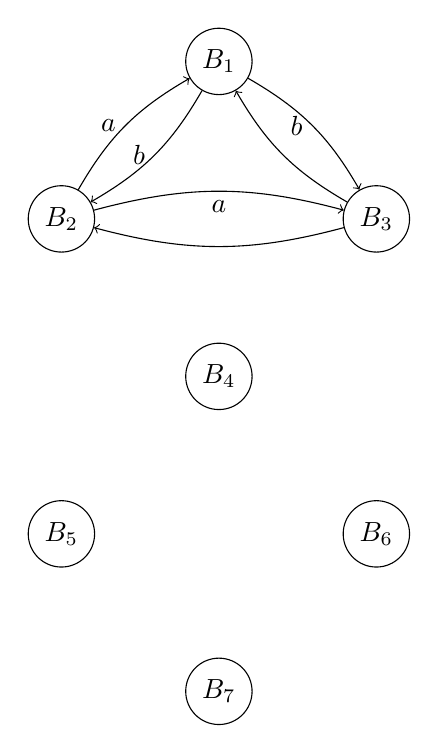
\begin{tikzpicture}
    \node[shape=circle,draw=black] (B1) at (0,0) {$B_1$};
    \node[shape=circle,draw=black] (B2) at (-2,-2) {$B_2$};
    \node[shape=circle,draw=black] (B3) at (2,-2) {$B_3$};
    \node[shape=circle,draw=black] (B4) at (0,-4) {$B_4$};
    \node[shape=circle,draw=black] (B5) at (-2,-6) {$B_5$};
    \node[shape=circle,draw=black] (B6) at (2,-6) {$B_6$};
    \node[shape=circle,draw=black] (B7) at (0,-8) {$B_7$};

    \path [->] (B1) edge[bend left=15] node[left] {$b$} (B2);
    \path [->] (B2) edge[bend left=15] node[left] {$a$} (B1);
    
    \path [->] (B1) edge[bend left=15] node[left] {$b$} (B3);
    \path [->] (B3) edge[bend left=15] node[left] {$\varnothing$} (B1);
    
    \path [->] (B3) edge[bend left=15] node[above] {$\varnothing$} (B2);
    \path [->] (B2) edge[bend left=15] node[below] {$a$} (B3);

\end{tikzpicture}
    \caption{The GNBA for $\phi \eqdef true\U (a \land b)$.}
    \label{fig:gnba-example1}
\end{figure}
\end{example}

\subsection{NBA}\label{sec:nba}
The NBA is derived from the GNBA by a well-defined transformation. The equivalent NBA accepts the same language as the GNBA but simplifies the model checking algorithm. We say that for a GNBA $\mathcal{G}$ there exists a NBA $\mathcal{A}$ such that $\mathcal{L}_\omega(\mathcal{G})=\mathcal{L}_\omega(\mathcal{A})$. The transformation for $\mathcal{G}=(Q,\Sigma,\delta,Q_0,\mathcal{F})$ and $\mathcal{F}=\{F_1,\ldots,F_k\}$ is constructed by creating $k$ copies of the GNBA. Then, for the $i$th copy, the acceptance states are connected to the equivalent states in the $(i+1)$th copy. Because a run can only move from the $i$th copy to the next through an acceptance state $q \in F_i$, the construction ensures that an accepting run visits an acceptance state in each copy infinitely often. The construction of the NBA $\mathcal{A}=(Q',\Sigma',\delta',Q_0',F')$ is formalized as follows:

\begin{definition}[Construction of NBA from GNBA~{\cite[Thm.~4.56]{baier2008principles}}]
Given an GNBA an equivalent NBA can be constructed in time and space $\mathcal{O}(|\mathcal{G}|\cdot|\mathcal{F}|)$. Let $\mathcal{G}=(Q,\Sigma,\delta,Q_0,\mathcal{F})$ with acceptance states $\mathcal{F}=\{F_1,\ldots,F_k\}$ then the NBA $\mathcal{A}=(Q',\Sigma',\delta',Q_0',F')$ can be constructed as:
\begin{itemize}
    \item $Q'=Q\times \{1,\ldots,k\}$,
    \item $Q_0'=Q_0 \times \{1\} = \{\langle q_0,1 \rangle \mid q_0 \in Q_0\}$, and
    \item $F'=F_1 \times \{1\} = \{\langle q_F,1 \rangle \mid q_F \in F_1\}$
\end{itemize}
With the transition relation:
\begin{equation*}
    \delta'(\langle q,i \rangle, A)=
    \begin{cases*}
      \{\langle q',i \rangle \mid q' \in \delta(q,A)\} & if $q \not\in F_i$ \\
      \{\langle q',i+1 \rangle \mid q' \in \delta(q,A)\}        & otherwise
    \end{cases*}
\end{equation*}
\end{definition}

\subsection{Product Automaton}
\label{sec:product-automaton}
The product automaton $TS \otimes A$ is constructed from the transition system $TS$ and the automaton $A$ over $\phi$ by constructing every possible pair of states from both systems with some relation function between states. This results in at most $|TS|\cdot |A|$ states. The intuitive understanding of the product is to combine all paths in $TS$ with all runs of $A$. The formal definition of the product automaton is given by:
\begin{definition}[Product of Transition System and NBA~{\cite[Def.~4.62]{baier2008principles}}]
Let $TS=\left( S, \longrightarrow, I, AP, L \right)$ be a transition system without terminal states and $\mathcal{A}=\left( Q, 2^{AP}, \delta, Q_0, F \right)$ a nonblocking NBA. Then, $TS \otimes \mathcal{A}$ is the following transition system:
\begin{align*}
    TS \otimes \mathcal{A} = \left( S \times Q, \longrightarrow', I', AP' \right)
\end{align*}
where $\longrightarrow'$ is the smallest relation defined by the rule
\begin{align*}
    \frac{s \longrightarrow t \land q \xrightarrow{L(t)} p}{ \langle s, q \rangle \longrightarrow' \langle t, p \rangle}
\end{align*}
and where
\begin{itemize}
    \item $I' = \{ \langle s_0, q \rangle \mid s_0 \in I \land \exists q_0 \in Q_0 . q_0 \xrightarrow{L(s_0)} q \}$,
    \item $AP' = Q$ and $L' : S \times Q \rightarrow 2^Q$ is given by $L'(\langle s, q \rangle) = \{q\}$.
\end{itemize}
Furthermore, let $P_{pers(\mathcal{A}}$ be the persistence property over $AP' = Q$ given by
\begin{align*}
    \text{"eventually forever $\lnot F$"}
\end{align*}
where $\lnot F$ denotes the propositional formula $\bigwedge\limits_{q \in Q} \lnot q$ over $AP' = Q$.
\end{definition}

The problem of checking $\phi$ is the reduced to checking whether $Traces(TS) \cap \mathcal{L_\omega}(A) \neq \varnothing$. We prove this by finding a path in the product for which an accepting state of $A$ is visited infinitely often. This path is then a counterexample for $TS \not\models \phi$. If no counterexample is found, then $\phi$ is proved to hold.

\subsection{Nested Depth-First Search}\label{sec:methods-ndfs}
The problem of determining $Traces(TS) \cap \mathcal{L_\omega}(A) \neq \varnothing$, as described above in \autoref{sec:product-automaton}, results in checking whether a path exists in $TS \otimes A$ which visits an acceptance state infinitely often. Finding such a path is achieved with a nested depth-first search (NDFS). The algorithm is structured as an outer and inner depth-first search (DFS) for which the outer DFS searches to find an accepting state and the inner DFS searches to find a cycle. If such a cycle can be found one can conclude that the accepting state can be visited infinitely often, proving $TS \not\models \phi$. If the outer DFS manages to explore all accepting states with no accepting cycles in the inner DFS, then no counterexample can be found, thus $TS \models \phi$ is proved.
\begin{algorithm}[H]
\SetAlgoLined
\DontPrintSemicolon
\SetKwProg{dfs}{Algorithm}{}{}
\dfs{dfs(s)}{
    $P = S \cup \{s, 0\}$\;
    $\textit{push}(S,s)$\;
    \For{$t \in successors(s)$}{
        \If{$\{t,0\} \not\in P$}{
            $\textit{dfs}(t)$
        }
        \If{$s \in acceptance$}{
            $\textit{ndfs}(s)$
        }
        $pop(T)$\;
    }
}{}\;

\SetKwProg{ndfs}{Procedure}{}{}
\ndfs{ndfs(s)}{
    $P = P \cup \{s, 1\}$\;
    $\textit{push}(T,s)$\;
    \For{$t \in successors(s)$}{
        \uIf{$t \in S$}{
            \KwRet true\;
        }\uElseIf{$\{t,1\} \not\in P$}{
            $\textit{ndfs}(t)$
        }
    }
    $\textit{pop}(T)$
}{}
\caption{Cycle detection algorithm using nested DFS.}
\label{alg:ndfs}
\end{algorithm}
In \autoref{alg:ndfs} the algorithm for NDFS can be seen, which is inspired by~\cite[Fig.~4]{holzmann1996nested}. The algorithm is structured as two recursive DFS algorithms, one for the outer and one for the inner DFS. The outer DFS will search recursively until no more successors can be recursed, then call the NDFS procedure on all acceptance states as the recursion unfolds. By postponing the inner DFS one can limit the number of states recursed by the inner DFS before finding a cycle, as the inner recursion searches until it hits the stack from the outer DFS, in which case a cycle has been found.